% !TEX root = ../notes_template.tex
\chapter{Discrete Math}\label{chp:discrete_math}
\minitoc
gls example
\begin{itemize}
	% \item \glsxtrshort{gcd};
	\item \Gls{gcd};
\end{itemize}

\section{Proof}
\begin{lemma}
\end{lemma}
\begin{claim}
\end{claim}
\begin{theorem}
\end{theorem}
\begin{example}
\end{example}
\begin{fact}
\end{fact}
\begin{remark}
\end{remark}
\begin{exercise}
	Prove
\end{exercise}
\begin{solution}
By induction:
\end{solution}

\lipsum % dummy text - remove from real document

\section{Quantifier}
\lipsum % dummy text - remove from real document

\section{Graph}
\citetitle{babaiGraphIsomorphismQuasipolynomial2016}
\cite{babaiGraphIsomorphismQuasipolynomial2016}

\section{Number theory}
Figure example
\begin{figure}[!ht]
    \centering
    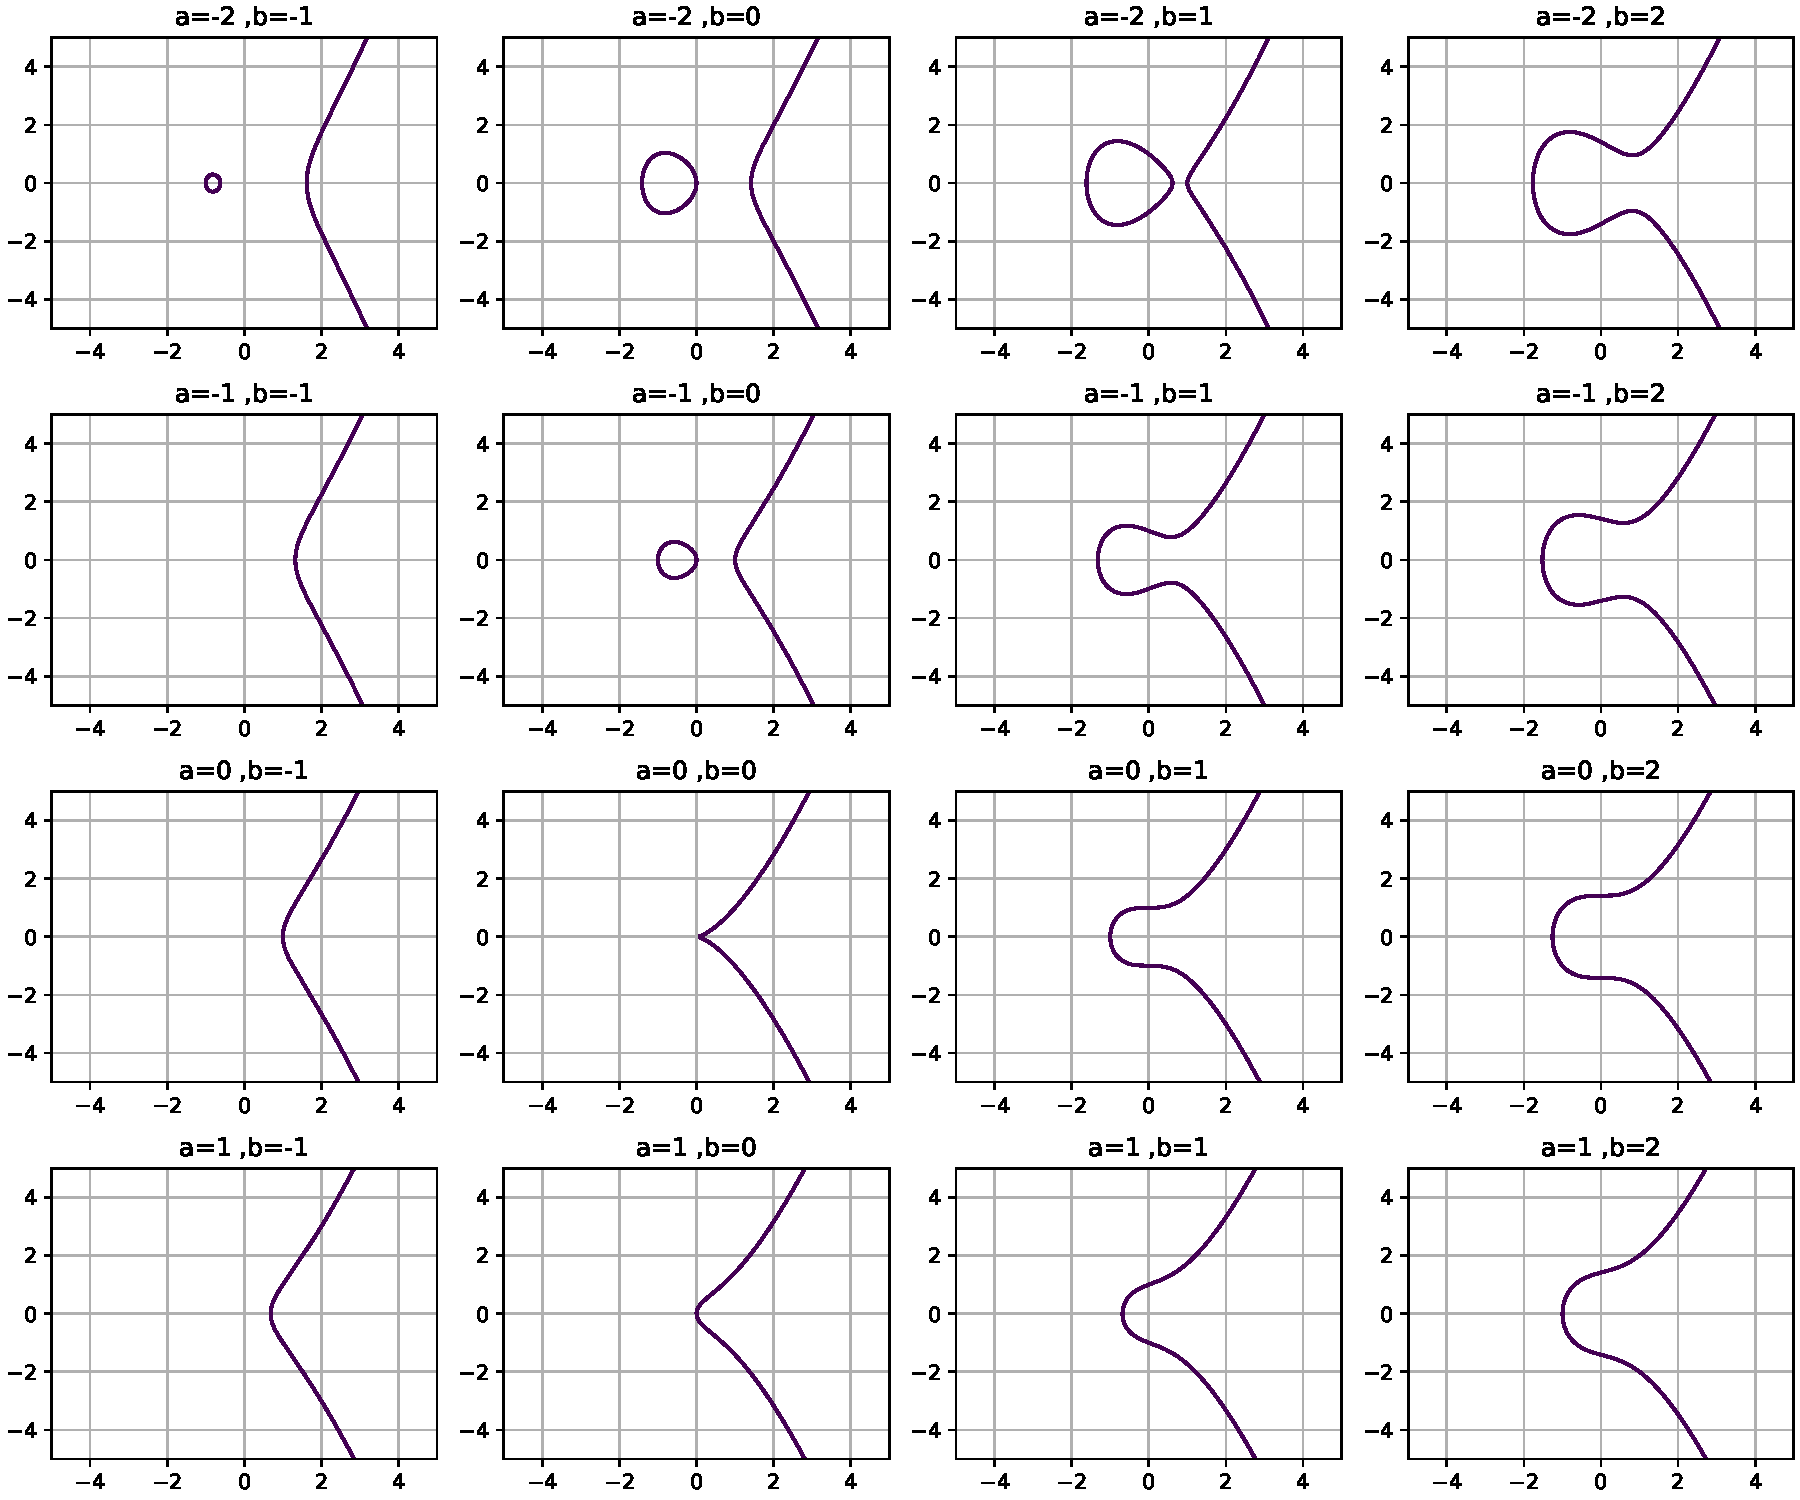
\includegraphics[width=1\linewidth]{./figure/elliptic_curves.pdf}
    \caption{Elliptic curves \cite{childsUniversalComputationQuantum2009} }
\end{figure}


\section{Algorithm}
% \begin{center}
% \begin{minipage}{.9\linewidth}
% algorithm2e
% https://www.overleaf.com/learn/latex/Algorithms#The_algorithm2e_package
\begin{algorithm}[H]
    \SetKwInOut{Input}{input}
    \SetKwInOut{Output}{output}
    \Input{Integer $N$ and parameter $1^t$}
    \Output{A decision as to whether $N$ is prime or composite}
    \BlankLine
    \For{ $i = 1,2, \ldots, t$} {
        $a\leftarrow \qty{1,\dots,N_1}$\;
        \If{$a^{N-1} \neq 1 \mod{N}$}
    {\Return "composite"}
    }
    \Return "prime"
    \caption{Primality testing - first attempt}
    \label{alg:miller_rabin}
\end{algorithm}
% \end{minipage}
% \end{center}